\documentclass[
	12pt,				% tamanho da fonte		
	oneside,
	a4paper,			% tamanho do papel.
	chapter=TITLE,
	sumario=tradicional,
	english,			% idioma adicional
	brazil,				% idioma principal do documento
	]{abntex2}

% ---
% PACOTES
% ---
\usepackage{lmodern}			% Usa a fonte Latin Modern
\usepackage[T1]{fontenc}		% Selecao de codigos de fonte.
\usepackage[utf8]{inputenc}		% Codificacao do documento (conversão automática dos acentos)
\usepackage{indentfirst}		% Indenta o primeiro parágrafo de cada seção.
\usepackage{color}				% Controle das cores
\usepackage{graphicx}			% Inclusão de gráficos
\graphicspath{{figuras/},{figuras/Intro/},{figuras/CAP2/},{figuras/CAP3/},{figuras/CAP4/},{figuras/CAP5/}}
\usepackage{microtype} 			% para melhorias de justificação
\usepackage{booktabs}
\usepackage{float} 				% Set posição da figura
\usepackage[bottom]{footmisc} 
\usepackage{subfig} 			% Inserir subfiguras
\usepackage[table,xcdraw]{xcolor} 	% Cor de preenchimento das tabelas
\usepackage{multirow} 			%mesclar cel em tabelas
\usepackage{verbatim}			%Inserir codigos fontes e comentários em massa
\usepackage[alf]{lib/abntex2cite}
\usepackage[brazilian,hyperpageref]{backref}
\usepackage{lipsum}				% para geração de dummy text
\usepackage{amsmath}
\usepackage[bottom]{footmisc}
\usepackage{footnote}
%\usepackage{fnpos}
%\usepackage{ftnxtra}
\usepackage{listings} 			%Inserir códigos fontes
\usepackage{rotating} 			%Rotação de páginas
\usepackage{placeins}			% Forçar o posicionamento da figura
\usepackage[top=3cm, bottom=2cm, left=3cm, right=2cm]{geometry} % Margens


% ---
% Informações de dados para CAPA e FOLHA DE ROSTO
% ---

\titulo{{\normalfont \textbf{Desenvolvimento de sistema de design e biblioteca de componentes para o Tribunal de Contas do Estado do Rio Grande do Norte}}}
\autor{Alvaro Portela Figueiredo Neto}
\local{Natal -- RN}
\data{Dezembro de 2020}
\instituicao{
  Universidade Federal do Rio Grande do Norte -- UFRN
  \par
  Instituto Metrópole Digital -- IMD
  \par
  Residência em Tecnologia da Informação
}
\tipotrabalho{Relatório técnico}

\preambulo{Trabalho de Conclusão de Curso da Residência em Tecnologia da Informação do Instituto
Metrópole Digital da Universidade Federal
do Rio Grande do Norte.
\newline 
\newline 
Orientador: Itamir de Morais Barroca Filho}

% Configurações de aparência do PDF final
% alterando o aspecto da cor azul
\definecolor{blue}{RGB}{41,5,195}
% informações do PDF
\makeatletter
\hypersetup{
     	%pagebackref=true,
		pdftitle={\@title}, 
		pdfauthor={\@author},
    	pdfsubject={\imprimirpreambulo},
	    pdfcreator={LaTeX with abnTeX2},
		pdfkeywords={abnt}{latex}{abntex}{abntex2}{relatório técnico}, 
		colorlinks=true,       		% false: boxed links; true: colored links
    	linkcolor=black,          	% color of internal links
    	citecolor=black,        		% color of links to bibliography
    	filecolor=magenta,      		% color of file links
		urlcolor=blue,
		bookmarksdepth=4
}
\makeatother
% Espaçamentos entre linhas e parágrafos 
\setlength{\parindent}{1.25cm} % Tamanho do parágrafo
\setlength{\parskip}{0.2cm}	% Controle do espaçamento entre um parágrafo e outro

%\onelineskip % Controle do espaçamento entre um parágrafo e outro

\makeindex % compila o indice

% Início do documento
% ----
\begin{document}

% Seleciona o idioma do documento (conforme pacotes do babel)
%\selectlanguage{english}
\selectlanguage{brazil}

% Retira espaço extra obsoleto entre as frases.
\frenchspacing 

% ----------------------------------------------------------
% ELEMENTOS PRÉ-TEXTUAIS
% ----------------------------------------------------------
\pretextual

% Capa
\imprimircapa

% Folha de rosto
\imprimirfolhaderosto

% Inserir folha de aprovação
\begin{folhadeaprovacao}
	
	\begin{center}
		{\ABNTEXchapterfont\large\imprimirautor}
		
		\vspace*{\fill}\vspace*{\fill}
		\begin{center}
			\ABNTEXchapterfont\bfseries\Large\imprimirtitulo
		\end{center}
		\vspace*{\fill}
		
		\hspace{.45\textwidth}
		\begin{minipage}{.5\textwidth}
			\imprimirpreambulo
		\end{minipage}%
		\vspace*{\fill}
	\end{center}
	
	Trabalho aprovado. \imprimirlocal, 29 de Janeiro de 2021:
	
	
	\setlength{\ABNTEXsignwidth}{14cm}
	\assinatura{\textbf{Prof. Dr. Itamir de Morais Barroca Filho - Orientador} \\ UFRN} 
	\assinatura{\textbf{Prof. Dr. Jair Cavalcanti Leite} \\ UFRN}
	\assinatura{\textbf{MSc. André Gustavo Almeida e Silva} \\ TCE-RN }
	
	\begin{center}
		\vspace*{0.5cm}
		{\large\imprimirlocal}
		\par
		{\large\imprimirdata}
		\vspace*{1cm}
	\end{center}
	
\end{folhadeaprovacao}

% ---
% Dedicatória
% ---
% \begin{dedicatoria}
% 	\vspace*{\fill}
% 	\centering
% 	\noindent
% 	\textit{Escreva aqui sua dedicatória}
% 	 \vspace*{\fill}
% \end{dedicatoria}

% Agradecimentos
% \begin{agradecimentos}
% Escreva aqui seus agradecimentos.

\end{agradecimentos}

% ---
% Epígrafe
% ---
% \begin{epigrafe}
% 	\vspace*{\fill}
% 	\begin{flushright}
% 		\textit{``Feliz o homem que encontrou a sabedoria e alcançou o entendimento,\\
% 			porque a sabedoria vale mais do que a prata, \\
% 			e dá mais lucro que o ouro."\\
% 			(Bíblia Sagrada, Provérbios 3, 13-14)}
% 	\end{flushright}
% \end{epigrafe}

% RESUMO
% resumo na língua vernácula (obrigatório)
\setlength{\absparsep}{18pt} % ajusta o espaçamento dos parágrafos do resumo
\begin{resumo}

É competência do Tribunal de Contas do Estado do Rio Grande do Norte (TCE-RN) o controle externo sobre a administração pública de acordo com o que rege a Constituição Federal de 1988, assim como a prestação de contas à sociedade das entidades jurisdicionadas sob sua guarda. Para a execução dessas ações o TCE-RN desenvolve e utiliza diversos Sistemas Web, seja para permitir que entidades jurisdicionadas  cadastrem ou acesse informações referentes ao escopo de interesses do TCE-RN ou permitir a divulgação de dados a população e aos Jurisdicionados como determinada pela Lei Complementar 131 também conhecida como Lei de Transparência. Diversos processos e tecnologias são usados no desenvolvimento dos sistemas do TCE-RN e o objetivo deste trabalho será introduzir um sistema de design de interfaces de usuário que seja ágil, colaborativo, versionável e adaptável, criando um conjunto componentes tanto para web quanto para dispositivos móveis.
%  \lipsum[1-1]
 
 \noindent
 \textbf{Palavras-chaves}: Sistemas de design. Biblioteca de componentes. Figma. 
\end{resumo}
% ---
% resumo em inglês
\begin{resumo}[Abstract]
	\begin{otherlanguage*}{english}
	
	The Court of Auditors of the State of Rio Grande do Norte (TCE-RN) is responsible for external control over public administration in accordance with the 1988 Federal Constitution, as well as the rendering of accounts to society of the jurisdicted entities under its guard. For the execution of these actions, TCE-RN develops and uses several Web Systems, either to allow jurisdicted entities to register or access information related to the scope of interests of TCE-RN or to allow the disclosure of data to the population and to jurisdicted's as determined by Law Complementary 131 also known as the Transparency Law. Several processes and technologies are used in the development of TCE-RN systems and the objective of this work will be to introduce a user interface design system that is agile, collaborative, versionable and adaptable, creating a set of components for both web and mobile devices. 
% 	\lipsum[1-1]
	
	\vspace{\onelineskip}
	\noindent 
	\textbf{Keywords}: Design System. Component Library. Figma.
	\end{otherlanguage*}
\end{resumo}

% ---
% inserir lista de ilustrações
\pdfbookmark[0]{\listfigurename}{lof}
\listoffigures*
\cleardoublepage

% inserir lista de tabelas
\pdfbookmark[0]{\listtablename}{lot}
\listoftables*
\cleardoublepage

% inserir lista de abreviaturas e siglas
\begin{siglas}
\label{ch:siglas}
	\item[TCE-RN] \textit{Tribunal de Contas do Estado do Rio Grande do Norte}
	\item[API] \textit{Application Programming Interface}
	\item[SIAI] \textit{Sistema Integrado de Auditoria Informatizada}
	\item[DIN] \textit{Diretoria de Informática}
	\item[IMD] \textit{Instituto Metrópole Digital}
	\item[HTML] \textit{HyperText Markup Language}
	\item[JSON] \textit{JavaScript Object Notation}
	\item[REST] \textit{Representational State Transfer}
	\item[Pencil] \textit{Pencil Project}
\end{siglas}

% inserir lista de símbolos
% \begin{simbolos}
%   \item[$ \Gamma $] Letra grega Gama
%   \item[$ \Lambda $] Lambda
%   \item[$ \zeta $] Letra grega minúscula zeta
%   \item[$ \in $] Pertence
% \end{simbolos}

% inserir o sumario
\pdfbookmark[0]{\contentsname}{toc}
\tableofcontents*
\cleardoublepage

\textual



% Capitulo 1: Introdução
\chapter[Introdução]{Introdução}
\label{ch:introducao}

  O Tribunal de Contas do Estado do Rio Grande do Norte (TCE-RN) segundo \cite{Legislativa} é o orgão responsavel pelo controle externo do Poder Legislativo Municipal, cabendo a este o parecer à prestação de contas que as prefeituras ou qualquer outro orgão sob sua jurisdição deve prestar anualmente.

  A exceção dos dados sob sigilo ou restrições da lei nº 12.557 \cite{lei_12527} é dever do Poder Executivo Federal promover a cultura de transparência pública a publicação de dados contidos em bases de dados de orgãos e entidades da administração pública federal direta, autárquica e fundacional sob a forma de dados abertos assim como fomentar o controle social e o desenvolvimento de novas tecnologias destinadas à construção de ambiente de gestão pública participativa e democrática e à melhor oferta de serviços públicos para o cidadão \cite{dec_8777}.

  Embora seja um tribunal o Tribunal de Contas não encontra-se circunscrito nem faz parte do Poder Judiciário, pois seu caráter é de naturazea, administrativa (contábil), trabalhando em parceria e nao em subordinação ao  ao Judiciário \cite{barreto_tribunais}.
  
  Portanto como corte cuja finalidade é a fiscalização de Prefeituras dos Municípios o TCE-RN 

\section{Uma subseção explicativa}

Lorem ipsum, uma citação direta 



Para compreender melhor as grandes mudanças e os benefícios gerados pelas \textit{Smart Grids} no contexto do fornecimento elétrico, a \autoref{tab-comparativa} traz um breve comparativo entre as redes tradicionais e as redes inteligentes.



\section{Trabalhos Relacionados}
\lipsum[1-1]

\section{Motivação}
O que lhe motiva a realizar este trabalho.

\section{Objetivos}
Objetivo geral e específicos.

\section{Estrutura do Trabalho}
Este trabalho apresenta uma introdução sobre o tema, mostrando os fatores que motivam a implantação da ideia, além da justificativa e dos objetivos. Em sequência, o \autoref{ch:cap2} aborda (...). O \autoref{ch:cap3}, por sua vez, explica a metodologia para ..., enquanto o \autoref{ch:cap4} trata de (...). O \autoref{ch:cap5} apresenta (...). Por fim, o \autoref{ch:cap6} traz as principais conclusões e contribuições deste trabalho.


% Capitulo 2
% \chapter[Capítulo 2]{Estado da Arte e Fundamentação Teórica}
\label{ch:cap2}

  Neste capítulo será apresentado o estado da arte referente a construção de sistemas de designs e prototipação, assim como o material utilizado como embasamento teórico para o seu desenvolvimento.

\section{Afinal o que é um sistema de design}
  Realizando uma breve pesquisa na internet a expressão mais comumente encontrada para descrever o que seria um sistema de design remetem a Nathan Curtis e a frase \textit{"A Design System isn’t a Project. It’s a Product, Serving Products".} \cite{descricao_sistema_design} Poderiamos traduzir para Um sistema de design não é um projeto. É um produto servindo outros produtos.

  Um sistema de design é a representação viva de um conjunto de documentos com o intuito de unificar a identidade visual de um ecossistema de produtos de uma instituição. Para servir a este propósito esses documentos não podem ser estáticos, devem permitir constantes mudanças e conseguir manter a ideia central de poder encaixar formas sem perder consistência \cite{design_gov_digital}.
  Em 2019, o Governo Federal decidiu iniciar a construção do seu sistema  de design com uma motivação clara

\begin{citacao}[brazil]
  [...]A iniciativa potencializa a eficiência e a eficácia dos usuários na utilização de interfaces para acesso aos serviços e aos sistemas de Governo, possibilitando uma única curva de aprendizado e garantindo a previsibilidade na utilização dos diferentes sistemas. \cite{design_gov_federal}
\end{citacao}

  Para Gonzalez um sistema de design é "[...]um conjunto de padrões para design e código, componentizado que unificam as duas práticas". \cite{GuilhermeGonzalez} Para o Governo Federal um \textit{Design System} "[...]tem como objetivo guiar todos os responsáveis pela construção de interfaces interativas orientadas à experiência única do usuário, considerando a acessibilidade e a usabilidade dos sistemas". \cite{design_gov_federal}

  É fato que grandes entidades vêm adotando a elaboração de sistemas de design com o intuito de se beneficiar das vantagens proporcionadas pela unificação da linguagem unificada de comunicação com usuários de seus sistemas, acelerar o processo de prototipação de seus layouts e interfaces e, deminuir o tempo de desenvolvimento das aplicações por meio do respaldo de bibliotecas de componentes mantidas por esses sistemas.

  Para citar algumas das empresas e entidades que possuem ou estão em processo de desenvolvimento de um sitema de design:

\begin{itemize}
  \item \href{https://material.io/design/}{Google}
  \item \href{https://www.microsoft.com/design/fluent/#/}{Microsoft}
  \item \href{https://developer.apple.com/design/}{Apple}
  \item \href{https://www.carbondesignsystem.com/}{IBM}
  \item \href{https://www.figma.com/community/plugin/860845891704482356/GitLab}{GitLab}
  \item \href{https://www.gov.br/governodigital/pt-br/transformacao-digital/ferramentas/design-system}{Governo Federal}
  \item \href{https://www.gov.uk/guidance/government-design-principles}{Governo do Reino Unido }
  \item \href{https://designsystem.gov.au/}{Governo da Australia}
\end{itemize}

\section{Principios e Tecnologias usadas para desenvolver um sistema de design}

  Existem uma quantidade virtualmente infinita de maneiras de se construir um \textit{Design System}. Contudo uma das maneiras mais comuns de se proceder com seu desenvolvimento consiste em separar o conjunto de documentos gerados, agrupando-os em categorias de acordo com a sua finalidade.

  No caso do Governo Fedaral, por exemplo, temos seu sistema de design separado em: Fundamentos Visuais, Componentes, Templates, Guias e Orientações. Esta separação foi feita com o intuito de melhor guiar a decisões de design, ser autênticos e específicos, em vez de genéricos e ser facilmente memorizáveis, fáceis de lembrar e utilizáveis no dia a dia. \cite{design_gov_federal}

  o Gitlab por sua vez optou por uma estrutura organizacional de seu sistema em: Fundação, Layout, Componentes, Visualização de dados, Regiões, Objetos, Conteúdo, Usabilidade e Recursos de Design. Para a equipe do GitLab o foco era que a companhia precisaria informar seus princípios, valores e propósito, promover a produtividade e promover empatia \cite{gitlab_design}.

  A Microsoft vem passando sucessivas mudanças. Com um grande leque de produtos que variam de serviços de nuvem a sistemas operacionais para dispositivos embarcados, unificar uma linguagem de comunicação sempre foi um problema para esta empresa. Atualmente, um dos foco da microsoft vem sendo o desenvolvimento de um linguagem visual chamada Fluent Design com o intuito criar engajamento e permitir accesibilidade e internacionalização em um ecossistema de programas e serviços focados em produtividade que se estende por múltiplas plataformas e sistemas operacionais. Separando inicialmente seu protuto por diferentes plataformas. Seu projeto de design se organiza em elementos básicos, layout, controles, estilo, movimento, "casca".

\begin{citacao}[brazil]
  Fluent experiences listen and adapt. They feel natural on the devices people use, from tablets to laptops, from PCs to televisions. They travel from the office to the living room to virtual worlds \cite{microsoft_fluent}.
\end{citacao}

  Estruturas de organização semelhantes se repetem e podem ser encontradas nos sistemas de design desenvolvidos, ou em desenvolvimento, de todas as empresas citadas na listagem da seção anterior.

  O agrupamento desses documentos são ações subjetivas e que devem ser executadas em parceria e comum acordo entre a equipe de design e de desenvolvimento. A categorização de estilos e componentes precisa não somente manter uma identidade visual única através das suas diferentes categorizações como fazer sentido de modo facilitar a sua executabilidade pelos desenvolvedores.

  Essa abordagem conjunta é importante, pois o desenvolvimento de um sistema de design em silos isolados por designers resulta em: Desperdício  de tempo e recursos humanos, sentimentos negativos e falta de compreensão sobre o design proposto \cite{GuilhermeGonzalez}. É possivel estrapolar facilmente esta mentalidade de crescimento de membros de uma euipe para a quantidade de equipes num projeto.

  Softwares são muitas vezes construidos por times, que podem variar de times pequenos até equipes muito grandes e a medida que cresce a quantidade de membros em um time cresce a dificuldade em manter uma experiência de usuário coesa, pois cada pessoa traz opiniões e soluções com estilos diferentes que irão facilmente divergir \cite{airbnb_medium}

  Para promover essa integração entre desenvolvedores e designers, ferramentas de desenvolvimento e comunicação são utilizadas para não só construir e manter, mas também para compartilhar e compreender as decisões e práticas adotadas. Dentro do vasto conjunto de ferramentas existentes para tal, podemos citar algumas das mais conhecidas:

\begin{itemize}
  \item \href{https://www.sketch.com}{Sketch}
  \item \href{https://www.adobe.com/br/products/xd.html?promoid=3NQZBBTZ&mv=other}{AdobeXD}
  \item \href{https://www.figma.com/}{Figma}
  \item \href{https://www.invisionapp.com/studio}{Studio}
  \item \href{https://pencil.evolus.vn/}{Pencil}
  \item \href{https://balsamiq.com/wireframes/}{Balsamiq}
\end{itemize}

  Vale salientar que as ferramentas anteriormente citadas são usadas principalmente para prototipação e não são as únicas existentes no mercado, mas algumas das principais. Quanto a prototipação, ela é uma das etapas dos processos envolvidos no desenvolvimento de um produto e é fundamental, pois acelera etapas de validação e na consolidação de alguns elementos obtidos durante o levantamento de requisitos.

  Os protótipos criados podem ser de baixa ou alta fidelidade, estes termos de qualificação servem para descrever a distância obtida pela aparência ou comportamento entre o protótipo e o produto final a ser desenvolvido e não é incomum serem usados ambos, em diferentes etapas do processo de desenvolvimento do sistema ou da prototipação dependendo de quão avançado está a validação ou quão refinado deseja-se descrever o comportamento do sistema ou serviço.

  \begin{table*}[!htbp]
    \centering
    \caption{Vantagens e desvantagens do nível de fidelidade de protótipos}
    \begin{tabular}{|c|l|l|}
    \hline
    \rowcolor[HTML]{DDDDDD}
    Fidelidade &
      Vantagens &
      Desvantagens \\ \hline
    Baixa &
      \begin{tabular}[c]{@{}l@{}}Baixo custo de desenvolvimento\\ Avaliação de múltiplos conceitos\\ Aponta problemas de telas\\ Prova de conceito\end{tabular} &
      \begin{tabular}[c]{@{}l@{}}Checagem de erro limitada\\ Especificação de detalhamento pobre\\ Voltado ao facilitador\\ Sem valor após especificação de requisitos\\ Valor limitado para testes de usabilidade\\ Fluxo e navegação limitados\end{tabular} \\ \hline
    Alta &
      \begin{tabular}[c]{@{}l@{}}Funcionalidade Completa\\ Interativo\\ Voltado ao usuário\\ Esquema de navegação claros\\ Permite testes exploratórios\\ Sensação do produto final\\ Atua como especificação viva\end{tabular} &
      \begin{tabular}[c]{@{}l@{}}Desenvolvimento mais custoso\\ Demorado para criar\\ Ineficiente para provas de conceito\\ Ineficiente para obtenção de requisitos\end{tabular} \\ \hline
    \end{tabular}
    \label{table-fideliade-alta-vs-baixa}
    \fonte{\cite{fideliade_alta_vs_baixa}}
  \end{table*}
  
  É comum que o desenvolvimento do sistema de design anteceda um passo de muita importância que é a codificação desse design, criando assim, uma biblioteca de componentes utilizáveis tanto para o desenvolvimento do protótipo como do produto. Todas as empresas e entidades citadas no início do capítulo possuem essa implementação em maior ou menor grau de cobertura dos componentes, algumas em diferentes linguagens de programação para uma ou mais plataformas, como a web ou mobile.
  O Tribunal de contas do estado conta com uma implementação feita anteriormente a criação do sistema de design e com ajuda deste trabalho iremos ampliar o escopo dessa biblioteca.

% Capitulo 3
% \chapter[Capítulo 3]{Capítulo 3}
\label{ch:cap3}

Fórmulas e itens:

\begin{itemize}
    \item Primeiro
    \subitem - $C_1 > F_1 + F_2 $
    \item Segundo
    \subitem - $C_2 > F_1 + F_2 - C_1$
\end{itemize}

\begin{equation} \label{eq1}
R(t) = P(T > t) = 1 - F(t)
\end{equation}

\section{Seção 1} \label{secao1}

Use \textit{labels} para criar links para as seções, como \autoref{secao1}.

\lipsum[5-8]

% Capitulo 4
% \chapter[Capítulo 4]{Resultados Obtidos}
\label{ch:cap4}

  Ao final deste trabalho obtivemos a construção de um sistema de design usando a ferramenta Figma. Este SD não só contem os principais elementos usados atualmente na biblioteca de front-end, escrita em Angular, pelo Tribunal de contas do Estado do Rio Grande Do Norte como tambem inclue algumas sugestões de melhoria e evolução para esta biblioteca, permitindo que com algumas alterações a mesma possa manter uma identidade visual mais consistente entre seus sistemas a serem desenvolvidos no futuro e permita aos usuários manter uma experencia mais uniforme ao transitar entre sistemas mantidos ou desenvolvidos pelo TCE-RN.
  
  Alem disso a bibiliteca de componentes é graças ao uso do Figma versionavel dentro da propria ferramenta, permitindo que evoluções na identidade visual não se tornem incompativeis com sistemas existentes em situação legada. O versionamento dessas versões é feito por meio da publicação de alterações em um padrão muito parecido com o utilizado pela ferramente de versionamento de codigo usada pelo tribunal, o GitLab

  O Sistema de Design desenvolvido permite por meio do uso de instâncias de componentes preexistentes sejam criados protótipos de tela de alta fidelidade de maneira rapida e eficiente, permite tambem que os protótipos sejam testados por meio de fluxo de telas associados a ações disparadas por componentes, garantindo durante a fase de levantamento de requisitos usuariso sintam uma experiencia mais proxima da real seja testando um sistema ou uma nova funcionalidade em desenvolvimento.

  Alem disso a biblioteca de componentes pode ser compartilhada publicamente permitindo a qualquer cidadão com interesse de desenvolver alguma funcionalidade ou sistema que consuma dados fornecidos pelo TCE-RN mantenha a mesma conformidade com a identidade visual dos sistemas produzidos pelo Tribuinal de Contas.

  Contudo o sistema carece de testes de uso mais extensivos por parte dos desenvolvedores do TCE-RN não só para assegurar e cobrir eventuais falhas mas tambem para assegurar o treinamento dos desenvolvedores e lideres de projetos no uso de protótipos mas tambem na cultura de prototipação antes do desenvolvimento, de modo a permitir que mudanças em fazes iniciais da construção e testes de sistemas e funcionalidades causem um impacto menor no tempo de produção dos mesmos.

% \lipsum[3-5]
 
% \section{Seção}

% \section{Seção 2}\label{secao2}

% O SHAPE é a sigla em inglês para \textit{Symbolic Hierarchical Automated Reliability and Performance Evaluator}. Veja a \autoref{fig:sharpe}.

% \begin{figure}
% 	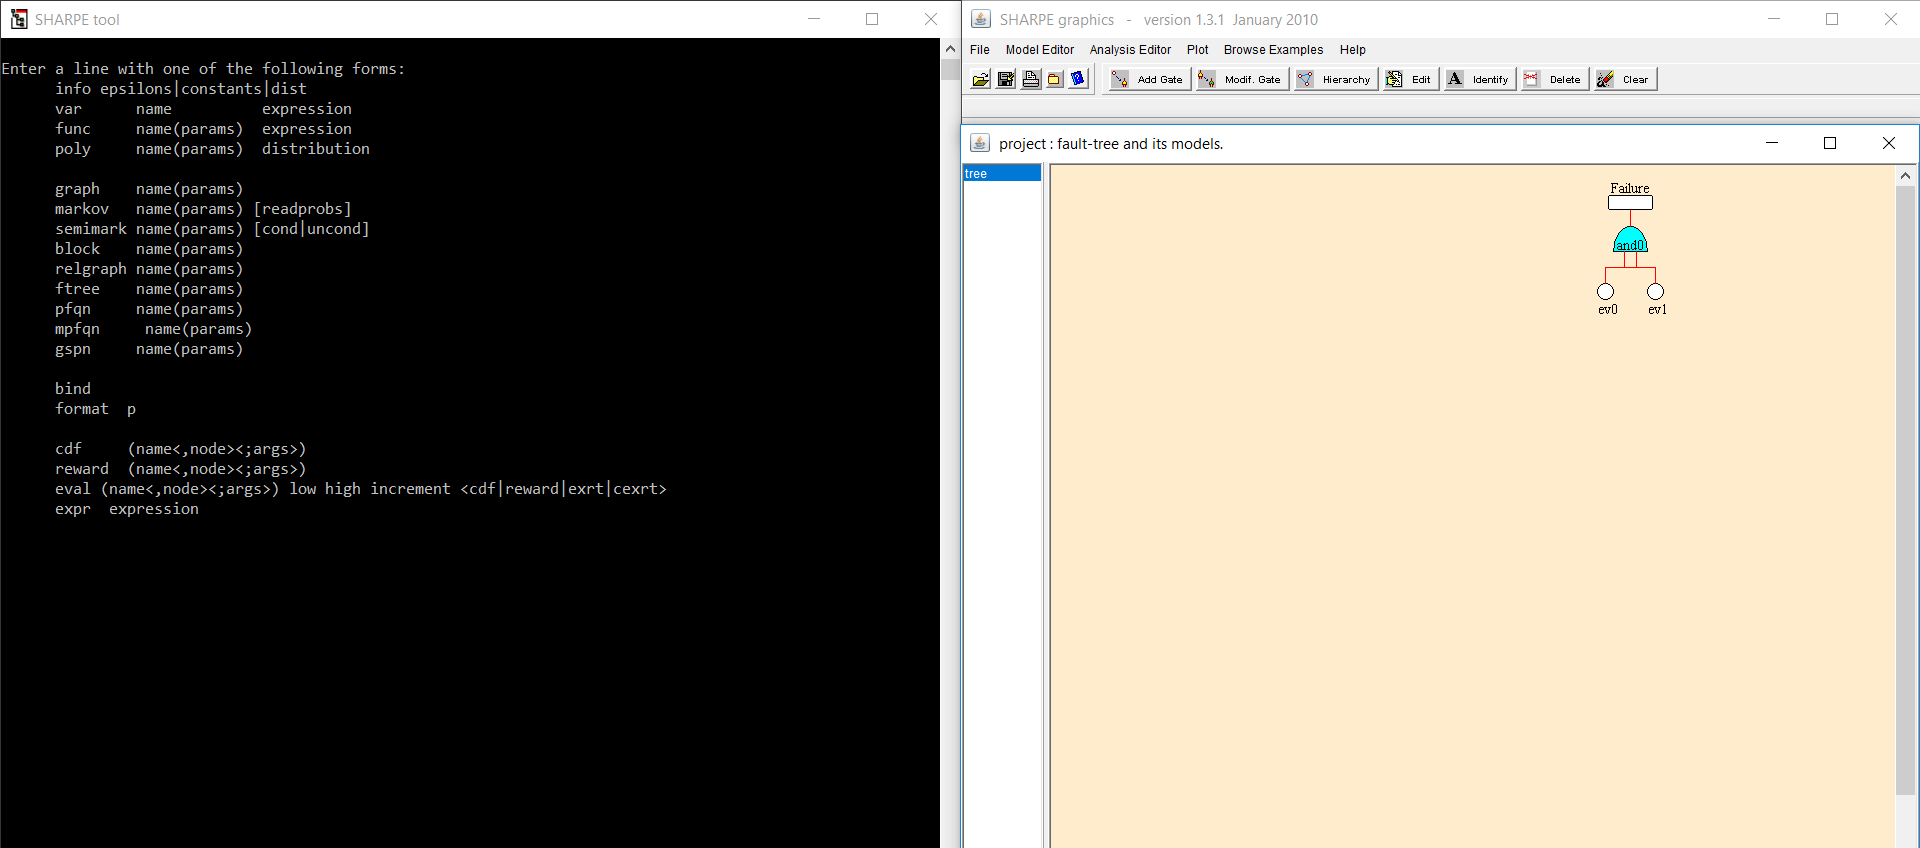
\includegraphics[width=1.0\textwidth, keepaspectratio=true]{sharpe}
% 	\centering
% 	\caption[\textit{Print screen} do SHARPE em linha de comando e em interface gráfica.]{\textit{Print screen} do SHARPE em linha de comando e em interface gráfica.}
% 	\fonte{Elaborada pela autora.}
% 	\label{fig:sharpe}
% \end{figure}

% Capitulo 5
% \chapter[Capítulo 5]{Conclusões e Propostas de Melhorias}
\label{ch:cap5}

  Neste capítulo trago minhas considerações finais sobre o qe foi alcançado e propostas para o amadurecimento do que foi desenvolvido.

\section{Conclusões}\label{cap5:conclusao}

  É fato que um sistema de design é um documento vivo e em evolução permanentemente e com este trabalho foi possivel realizar o desenvolvolvimento de um SD com a sobriedade, a objetividade e o senso de proposito pertinente ao Tribunal de Contas do Estado do Rio Grande do Norte, sendo assim é considerado pelo autor que as intenções e objetivos do trabalho foram alcançados com exito, evidentemente não sem sacrificios em relação as escolhas adotadas pois o desenvolvimento de um sistema de design não é algo que se conclui, mas que se abandona, pois o fim dos prazos chegam e o produto precisa ser entregue de um geitou ou de outro mas sempre passivel de melhorias, criticas e reenterpretações. Neste trabalho não foi diferente e apesar do desejo de continuar a evolução do que vinha-se desenvolvendo a entrega tinha que ser efetuada.

\section{Melhorias}\label{cap5:melhorias}

  Dentro das muitas melhorias possiveis, planejadas ou simplesmente encontradas podemos destacar acima de tudo a falta de comunicação direta com a biblioteca de componentes de front-end tce-ng-lib. Era esperado que as alterações propostas fossem incluidas nos componentes de front-end e a nomenclatura e descrição das duas poderiam ser melhoradas para entrar em conformidade tornando a busca e compreensão facilitadas. Outro grande problema foi a ausencia de um conjunto de componentes para dispositivos moveis, que foi pensado em se fazer inicialmente mas o estudo e preparatorio e as sucessivas revisões do trabalho consumiram muito tempo e o medo de nao conseguir terminar os documentos a tempo inibiram o inicio desta fase do trabalho.

  % \section{Melhorias}\label{cap5:melhorias}

% Conclusão
% \chapter[Conclusão]{Conclusão}
\label{ch:cap6}

Escreva suas conclusões, limitações do seu trabalho, contribuições, trabalhos futuros, etc.

% Capitulo guia 
% TODO remove this
\chapter[Roteiro]{guia}
\label{ch:guia}
O trexo abaixo sere ao proposito apenas de referencia a construcao desse documento e nao sera incluido em sua versao final

1 INTRODUCAO
    1.0 contextualizacao
    1.1 problema
        . transparencia
        . consumo mobile
        . quantidade de projetos
        . ferrametnas desatualizadas
    1.2 solucao
        . ferramenta moderna
        . baseada na web
        . colaborativa
    1.3 organizacao

2 Departamento de Informatica
    1.0 contextualizacao
    2.1 projetos e crescimento
    2.2 parceria com o IMD
    2.3 Estrutura de Trabalho Atual (Pencil)

% como montar referencias
links de construção de referencias:

https://zbib.org

https://truben.no/latex/bibtex/


% ----------------------------------------------------------
% ELEMENTOS PÓS-TEXTUAIS

% 
\postextual

% Referências bibliográficas
%\addcontentsline{toc}{chapter}{Referências Bibliográficas}

\bibliographystyle{abntex2-alf}
%\bibliographystyle{unsrt}
\bibliography{bibliografia/referencias}

\end{document}
